\documentclass[twoside]{article}
\usepackage{aistats2027}
\usepackage{amsmath,amssymb,amsthm,mathtools,bm}
\usepackage{booktabs,array,enumitem,microtype,graphicx,longtable,xcolor}
\usepackage{placeins}
\usepackage[hidelinks]{hyperref}
\graphicspath{{figures/}{./}}

\newtheorem{theorem}{Theorem}
\newtheorem{proposition}[theorem]{Proposition}
\newtheorem{lemma}[theorem]{Lemma}
\newtheorem{corollary}[theorem]{Corollary}
\newtheorem{property}[theorem]{Property}
\theoremstyle{definition}
\newtheorem{assumption}[theorem]{Assumption}
\newtheorem{definition}[theorem]{Definition}
\newtheorem{remark}[theorem]{Remark}

\newcommand{\Pp}{\mathbb P}
\newcommand{\E}{\mathbb E}
\newcommand{\KL}{\operatorname{KL}}
\newcommand{\kl}{\operatorname{kl}}
\newcommand{\Ber}{\operatorname{Ber}}
\newcommand{\1}{\mathbf 1}
\newcommand{\cP}{\mathcal P}
\newcommand{\argmax}{\operatorname*{arg\,max}}
\newcommand{\argmin}{\operatorname*{arg\,min}}
\newcommand{\GammaE}{\Gamma_{\beta}^{\mathrm E}}
\newcommand{\GammaU}{\Gamma_{\beta}^{\mathrm U}}
\newcommand{\Ldelta}{L_\delta}
% Shared notation used by the optional combined appendix.
\newcommand{\R}{\mathbb R}
\newcommand{\N}{\mathbb N}
\newcommand{\Ptheta}{\mathbb P_{\theta}}
\newcommand{\Etheta}{\mathbb E_{\theta}}
\newcommand{\ind}{\mathbf 1}
\newcommand{\cS}{\mathcal S}
\newcommand{\calP}{\mathcal P}
\newcommand{\calD}{\mathcal D}
\newcommand{\calO}{\mathcal O}
\newcommand{\calF}{\mathcal F}
\newcommand{\calI}{\mathcal I}
\newcommand{\Alt}{\mathrm{Alt}}
\newcommand{\GU}{\Gamma_{\beta}^{U}}
\newcommand{\TU}{T_{\beta}^{U}}
\begin{document}

\twocolumn[
\aistatstitle{Best-Arm Identification under One-Bit Threshold Feedback}
\aistatsauthor{Anonymous Author}
\aistatsaddress{Anonymous Institution}
]


\begin{abstract}
We study fixed-confidence best-arm identification when each reward is observed
only through a one-bit threshold comparison. We consider two observation
models. In Model E, rewards belong to a regular one-parameter exponential
family and the learner adaptively chooses the threshold. In Model U, each arm
has an arbitrary distribution supported on $[0,B]$, while an independent
uniform threshold is revealed together with the comparison bit.

For both models, we derive instance-dependent information-theoretic lower
bounds and construct fixed-$\beta$ Top-Two procedures whose leading expected
sample complexity matches these bounds. Here, fixed-$\beta$ means that
asymptotically a prescribed fraction $\beta\in(0,1)$ of samples is allocated
to the best arm, while the remaining samples are allocated to challengers.
For Model E, the optimal information allocation is a single feasible
arm--threshold design shared across all challengers. For Model U, the identity
$Y\sim\operatorname{Ber}(\mu/B)$ provides a distribution-free statistic for
identifying the leader, while the revealed thresholds retain additional
information that is used for challenger selection and stopping.

Beyond first-order asymptotic optimality, we establish finite-confidence
guarantees. A separate Model-E companion procedure admits an expected
stopping-time bound with leading term proportional to $\log(1/\delta)$ and
an explicit
$O\!\left(\log^{2/3}(1/\delta)
\sqrt{\log\!\left(e+\log(1/\delta)\right)}\right)$ correction, up to
lower-order terms. For the exact certified Model-U rule, we
obtain a leading $\log(1/\delta)$ term with an explicit
$O\!\left(\log^{3/4}(1/\delta)
\log^{3/2}\!\left(e+\log(1/\delta)\right)\right)$ correction for arbitrary
$[0,B]$-supported laws with interior means, without full-support or
global-slope assumptions. Experiments compare one-bit and full-feedback
sample complexities and evaluate the finite-confidence behavior of the
proposed procedures.
\end{abstract}

\section{INTRODUCTION}

Best-arm identification (BAI) asks a learner to identify the arm with the
largest mean while controlling the probability of a wrong recommendation.
In the fixed-confidence setting, the learner is given a risk level
$\delta\in(0,1)$ and chooses a data-dependent stopping time
$\tau_\delta$ such that the recommended arm is incorrect with probability at
most $\delta$. Under full feedback, the optimal first-order sample complexity
is characterized by change-of-distribution information, and asymptotically
optimal procedures are known for broad classes of bandit models
\cite{KCG2016,Jourdan2022}.

We study a more restrictive feedback model. After sampling an arm with reward
$X$, the learner does not observe $X$ itself, but only the comparison bit
\[
Y=\mathbf 1\{X\ge q\},
\]
where $q$ is a threshold. The choice, or generation, of $q$ is therefore part
of the statistical experiment.

We consider two models. In \emph{Model E}, each arm belongs to a regular
one-parameter exponential family and the learner adaptively chooses the
threshold $q$. In \emph{Model U}, an arm may have any probability law
supported on $[0,B]$; after the arm is selected, an independent threshold
$Q\sim\operatorname{Unif}[0,B]$ is generated and both $Q$ and the bit
$Y=\mathbf 1\{X\ge Q\}$ are revealed. Model U therefore provides a
\emph{current-status observation}: rather than observing the value of $X$, we
learn only whether $X$ lies above or below a revealed inspection threshold.

A key identity in Model U is
\[
\Pr(Y=1)
=
\frac{1}{B}\int_0^B\Pr(X\ge q)\,dq
=
\frac{\E[X]}{B}.
\]
Hence marginally $Y\sim\operatorname{Ber}(\mu/B)$, so the bits alone provide
a distribution-free estimator of the arm mean. Conditioning on the revealed
threshold $Q$, however, retains more information about the survival function
$q\mapsto\Pr(X\ge q)$. Our algorithms use these two views for different
purposes: the marginal bits identify the empirical leader, whereas the richer
threshold-conditioned likelihood is used to compare the leader with its
challengers and to construct stopping evidence.

When $K>2$, the pairwise comparisons are statistically coupled: all
challengers reuse the same observations collected from the best arm. Thus,
optimizing a different best-arm threshold distribution separately for each
challenger can produce mutually incompatible pairwise designs. For Model E we
therefore optimize over a single feasible arm--threshold occupation measure
shared by all challengers. Its optimal worst-case information rate is the
\emph{characteristic value}; its reciprocal is the corresponding
\emph{characteristic time}, which determines the leading asymptotic number of
samples.

Our algorithms follow the Top-Two principle: at each round, one arm acts as a
current leader and another as its most informative challenger, and sampling is
split between them. In the fixed-$\beta$ version, a prescribed fraction
$\beta\in(0,1)$ is asymptotically assigned to the best arm and the remaining
fraction $1-\beta$ to challengers.

\paragraph{Contributions.}
\emph{Matching instance-dependent lower and upper bounds.}
For both observation models we derive $K$-arm change-of-distribution lower
bounds and construct fixed-$\beta$ Top-Two procedures whose leading expected
stopping times match the corresponding characteristic times. This yields an
explicit measure of the information loss caused by one-bit feedback through
the ratio
\[
\frac{T_{\beta,\mathrm{1b}}^\star}
     {T_{\beta,\mathrm{full}}^\star}.
\]
For Model E, the optimization uses one feasible threshold design shared by all
challengers. For Model U, we obtain an exact reduction of the population
pairwise transportation problem to a one-dimensional mean-separation problem.

\emph{Finite-confidence guarantees.}
We provide $\delta$-PAC stopping rules and non-asymptotic probability and
expected-time bounds. A separate Model-E global-design companion admits an
explicit correction of order
\[
L_\delta^{2/3}\sqrt{\log(e+L_\delta)},
\qquad
L_\delta:=\log(1/\delta),
\]
up to lower-order terms. For the exact certified Model-U procedure, the
corresponding correction is
\[
L_\delta^{3/4}\log^{3/2}(e+L_\delta)
\]
for arbitrary probability laws supported on $[0,B]$ with interior means,
without density, full-support, or global-slope assumptions.

\emph{Empirical comparison.}
Paired simulations compare full and one-bit feedback and examine practical
fixed-point predictors. The practical simulations are separated from the
paper-certified Model-U finite-sample calibration, whose sieve penalty is
deliberately conservative at moderate sample sizes.

\paragraph{Related work.}
Our analysis builds on BAI lower bounds and Top-Two methods
\cite{KCG2016,Russo2016,Jourdan2022,DKM2019}. One-bit mean and
quantile estimation, bit-constrained BAI, and classical current-status
likelihoods provide related tools but address different statistical
experiments \cite{KipnisDuchi2022,LauScarlett2026AISTATS,
LauScarlett2026Tail,Faizal2023ICQ,LauScarlett2025,
GroeneboomWellner1992,GMW2008}.


\paragraph{Concurrent one-bit BAI.}
Concurrent work by Luong et al.~\cite{Luong2026NearlyOptimal} studies
fixed-confidence BAI under adaptive one-bit set queries with only a finite-variance
assumption.  It develops a time-uniform one-bit mean-estimation primitive and
clipping-based BAI algorithms, together with a gap-adaptive upper bound and a
two-arm worst-case lower bound matching the leading gap dependence up to
lower-order iterated logarithms.  Its lower bound is a worst-case two-arm
construction rather than an exact $K$-arm instance-dependent characteristic;
the paper explicitly leaves the exact instance-dependent complexity of one-bit
BAI open.  Our setting and objective are complementary: under Model E and
Model U we characterize the exact fixed-$\beta$ first-order
instance-dependent complexity through observed-law KL information and construct
procedures attaining the corresponding characteristic times.

\section{PROBLEM FORMULATION}
\label{sec:problem}
\paragraph{Fixed-confidence objective.}
There are $K\ge2$ arms and the true instance has a unique best arm $i^\star$.  At each round the learner chooses an arm, receives a one-bit observation according to one of the models below, and may stop at a data-dependent time $\tau_\delta$.  We call an algorithm $\delta$-PAC if, for every admissible instance,
\begin{equation}
\Pp(\tau_\delta<\infty)=1,
\qquad
\Pp(\widehat i_{\tau_\delta}\neq i^\star)\le\delta.
\label{eq:pac}
\end{equation}
When only the second inequality is used for an arbitrary sampling rule, we call it an incorrect-stop probability bound.
Write
\[
\Ldelta:=\log(1/\delta).
\]
\paragraph{Divergence notation.}
For $p,r\in[0,1]$, let
\[
\kl(p,r)
:=
p\log\frac{p}{r}
+(1-p)\log\frac{1-p}{1-r}
\]
denote the binary Kullback--Leibler divergence, with the usual extended-value
conventions at $0$ and $1$.  For general probability laws $P$ and $Q$,
$\KL(P,Q)$ denotes their Kullback--Leibler divergence.  If $P$ and $Q$ admit
densities $p$ and $q$ with respect to a common dominating measure $\nu$, then
\[
\KL(P,Q)=\int p(x)\log\frac{p(x)}{q(x)}\,d\nu(x),
\]
with $\KL(P,Q)=+\infty$ when $P\not\ll Q$.  Thus $\kl$ is reserved for
Bernoulli parameters, whereas $\KL$ denotes divergence between general
probability laws.

Our first-order complexity is the ratio $\E[\tau_\delta]/\Ldelta$.  We study its limit as $\delta\downarrow0$.  Suboptimal arms are allowed to have equal means throughout.

\subsection{Model E: adaptive thresholds in an exponential family}
Arm $k$ has law $P_{\theta_k}$ from the canonical one-parameter exponential family
\begin{equation}
f_\theta(x)=\exp\{\theta x-b(\theta)\}h(x),\qquad \theta\in\Theta,
\label{eq:expfam}
\end{equation}
where $\Theta=[\theta_-,\theta_+]$ is compact, $b\in C^2(\Theta)$ and $b''>0$.  Hence the mean $b'(\theta)$ is strictly increasing and $i^\star=\argmax_k\theta_k$.  The learner chooses a threshold $q_t$ in a compact set $Q$ and observes only
\[
Y_t=\1\{X_t\ge q_t\},\qquad X_t\sim P_{\theta_{I_t}}.
\]
Write $p_q(u)=P_u(X\ge q)$ and
\begin{equation}
d_q(u,v)=\kl\!\left(p_q(u),p_q(v)\right).
\label{eq:dq-main}
\end{equation}
Thus $d_q(u,v)$ is the KL divergence between the two Bernoulli observations
induced at threshold $q$ under candidate parameters $u$ and $v$.
We assume $(q,u)\mapsto p_q(u)$ is continuous, continuously differentiable in $u$, bounded away from $0$ and $1$ on $Q\times\Theta$, and that the one-bit log likelihood is uniformly Lipschitz in $u$.  These compact regularity assumptions are sufficient for the finite-time likelihood control and uniform information separation used below.
The uniform bound applies to the entire \emph{admissible parametric
family} and the \emph{selected compact query set}; it is not the
mere pointwise condition $0<p_q(u)<1$.

For $a\in\Theta$, define the armwise one-bit log likelihood
\begin{equation}
\begin{aligned}
\ell_{n,k}(a)
&:=
\sum_{\substack{t\le n\\ I_t=k}}
\bigl[
Y_t\log p_{q_t}(a)
+(1-Y_t)\log(1-p_{q_t}(a))
\bigr],\\
L_n(u)&:=\sum_{k=1}^K\ell_{n,k}(u_k).
\end{aligned}
\label{eq:LE-main}
\end{equation}
Because the joint likelihood is separable across arms, define the armwise
MLE by the measurable deterministic rule
\[
\widehat\theta_k(n)
:=
\min\!\left(\argmax_{a\in\Theta}\ell_{n,k}(a)\right),
\qquad
\widehat\theta(n)
=
\bigl(\widehat\theta_1(n),\ldots,\widehat\theta_K(n)\bigr).
\]
The minimum selects the smallest maximizer whenever the MLE is not unique.

For an ordered pair $(i,j)$ define
\begin{equation}
\begin{split}
W_n^{\rm E}(i,j)=&\,\ell_{n,i}(\widehat\theta_i(n))
+\ell_{n,j}(\widehat\theta_j(n))\\
&-\sup_{u_i\le u_j}\{\ell_{n,i}(u_i)+\ell_{n,j}(u_j)\}.
\end{split}
\label{eq:WE-main}
\end{equation}
Thus $W_n^{\rm E}(i,j)$ is the generalized likelihood-ratio evidence against
the alternative that arm $j$ is at least as good as arm $i$: it compares the
unrestricted pairwise maximum likelihood with the best fit satisfying
$u_i\le u_j$.  Large values therefore provide evidence that arm $i$ is better
than arm $j$.

The global statistic for recommending arm $i$ is
\[
Z_i(n):=\min_{j\neq i}W_n^{\rm E}(i,j).
\]
The minimum appears because arm $i$ can be recommended only after it has
accumulated evidence against every challenger; hence $Z_i(n)$ is controlled by
the currently least-separated competitor.

\subsection{Model U: revealed uniform thresholds}
Arm $k$ has an otherwise arbitrary law $F_k$ supported on $[0,B]$,
with mean $\mu_k\in(0,B)$.  After the learner chooses arm $I_t$, nature draws
$Q_t\sim{\rm Unif}[0,B]$ independently of $X_t\sim F_{I_t}$ and reveals
\[
(Q_t,Y_t),\qquad Y_t=\1\{X_t\ge Q_t\}.
\]
If $S_F(q)=P_F(X\ge q)$, then
\begin{equation}
Y\sim\Ber(\mu(F)/B),\qquad
Y\mid Q=q\sim\Ber(S_F(q)).
\label{eq:two-views}
\end{equation}
Thus the bit marginal is exactly $\Ber(\mu(F)/B)$.  Consequently,
$B$ times the empirical bit mean is a distribution-free consistent estimator
of the arm mean; at each fixed local pull count it is also unbiased.  The full
observed pair has KL divergence
\begin{equation}
D_{\rm U}(F,G)=\frac1B\int_0^B\kl(S_F(q),S_G(q))\,dq.
\label{eq:DU-main}
\end{equation}
The first identity in \eqref{eq:two-views} will define the leader; the richer current-status likelihood associated with \eqref{eq:DU-main} will define the challenger and the stopping rule.
\paragraph{Regularity differs between the models.}
Model E assumes that its finite-dimensional Bernoulli probabilities are
uniformly interior on the compact parameter--query domain.  Model U
retains all $[0,B]$-supported arm laws and optimizes over unrestricted candidate
survival functions, which can equal zero or one.  Its profile analysis
therefore uses a \emph{common, horizon-dependent smoothing map} in the
proof, not an extra restriction on the statistical experiment; see
Lemma~\ref{lem:U-BV-profile} and the accompanying appendix remark.

\section{A $K$-ARM LOWER BOUND}
\label{sec:lower}
We state the change-of-measure argument once, for a generic one-bit experiment.
When arm $k$ is sampled with action $a$ (a threshold in Model E; only the arm
label in Model U), let $P^a_{\nu_k}$ denote the law of the resulting observed
one-bit datum.  For two candidate arm models $\nu_k$ and $\lambda_k$, define
\[
d_a(\nu_k,\lambda_k)
:=
\KL(P^a_{\nu_k},P^a_{\lambda_k}),
\]
the expected log-likelihood ratio contributed by one observation from arm $k$
under action $a$.  For a probability design $\rho$ over all arm-action pairs
and an alternative instance $\lambda$, set
\begin{equation}
\mathcal I(\nu,\lambda;\rho)=\sum_{k=1}^K\int d_a(\nu_k,\lambda_k)\,\rho_k(da).
\label{eq:genericI}
\end{equation}
Thus $\mathcal I(\nu,\lambda;\rho)$ is the average information gained per
sample for discriminating the true instance $\nu$ from $\lambda$ under design
$\rho$.
Let $\mathcal A(\nu)$ be the set of \emph{strict} alternatives having a unique best arm different from $i^\star$.  The lower bound below is stated for this strict set.  For the fixed-$\beta$ designs with positive best-arm mass used to identify
the matching characteristics, the supplement separately verifies the
strict-alternative/closed-order-reversal reduction. The generic lower
bound itself is stated directly for strict alternatives.

\begin{theorem}[$K$-arm action-space lower bound]
\label{thm:KLB}
For every $\delta\in(0,1/2)$ and every $\delta$-PAC algorithm with $\E_\nu[\tau_\delta]<\infty$,
\begin{equation}
\begin{aligned}
\E_\nu[\tau_\delta]\,\Gamma^\star(\nu)
&\ge \kl(1-\delta,\delta),\\
\Gamma^\star(\nu)
&=\sup_{\rho}\inf_{\lambda\in\mathcal A(\nu)}
\mathcal I(\nu,\lambda;\rho).
\end{aligned}
\label{eq:KLB}
\end{equation}
The ratio form follows when $\Gamma^\star(\nu)>0$; if it is zero,
no $\delta$-PAC algorithm has finite expected stopping time on $\nu$.
\end{theorem}

The quantity $\Gamma^\star(\nu)$ is the largest worst-case information rate
achievable by a feasible design, and $1/\Gamma^\star(\nu)$ is the
corresponding first-order characteristic time.

The proof takes the expected stopped occupation measure of the actual adaptive experiment and applies the bandit change-of-distribution inequality to each strict alternative.  The important point for $K>2$ is structural: there is a single measure $\rho$ before nature chooses the challenger.  Hence the same best-arm threshold stream must serve all pairwise tests.

Most Top-Two algorithms fix the asymptotic fraction $\beta\in(0,1)$ of best-arm samples.  Restricting the design in \eqref{eq:KLB} to mass $\beta$ on the best arm gives $\Gamma_\beta^\star(\nu)$.

\begin{corollary}[Fixed-$\beta$ lower bound]
\label{cor:betaLB}
Under the compactness and finite-KL continuity conditions verified for Models E and U in the supplement, suppose a family of $\delta$-PAC algorithms satisfies
\[
\frac{\E_\nu[N_{\tau_\delta,i^\star}]}{\E_\nu[\tau_\delta]}\longrightarrow\beta.
\]
Then
\begin{equation}
\liminf_{\delta\downarrow0}
\frac{\E_\nu[\tau_\delta]}{\Ldelta}
\ge \frac1{\Gamma_\beta^\star(\nu)}.
\label{eq:betaLB}
\end{equation}
with the convention $1/0=+\infty$.
\end{corollary}

\subsection{The two characteristic values}
For Model E, let $\mathcal D_\beta^b$ collect all nonnegative threshold
measures $\rho=(\rho_1,\ldots,\rho_K)$ with
$\sum_k\rho_k(Q)=1$ and $\rho_b(Q)=\beta$.
The pairwise scalar reduction proved in the supplement yields
\begin{equation}
\begin{aligned}
\GammaE(\theta)
&=\max_{\rho\in\mathcal D_\beta^{i^\star}}
\min_{\substack{j\ne i^\star\\x\in\Theta}}\\[-2pt]
&\quad\Bigl[\int_Qd_q(\theta_{i^\star},x)\rho_{i^\star}(dq)\\[-1pt]
&\qquad+\int_Qd_q(\theta_j,x)\rho_j(dq)\Bigr].
\end{aligned}
\label{eq:GammaE-main}
\end{equation}
The best-arm measure $\rho_{i^\star}$ is visibly shared across all challengers.

For Model U, define the one-sided observed transportation costs
\begin{align*}
K_{\rm U}^-(F,x)&=\inf_{G:\mu(G)\le x}D_{\rm U}(F,G),\\
K_{\rm U}^+(F,x)&=\inf_{G:\mu(G)\ge x}D_{\rm U}(F,G).
\end{align*}
Let $\mathcal W_\beta:=\{w_j\ge0:\sum_{j\ne i^\star}w_j=1-\beta\}$.
Then
\begin{equation}
\begin{aligned}
\GammaU(\mathbf F)
&=\max_{w\in\mathcal W_\beta}
\min_{j\ne i^\star}\inf_{x\in[0,B]}\\[-2pt]
&\quad\bigl[\beta K_{\rm U}^-(F_{i^\star},x)\\[-1pt]
&\qquad+w_jK_{\rm U}^+(F_j,x)\bigr].
\end{aligned}
\label{eq:GammaU-main}
\end{equation}
In \eqref{eq:GammaU-main}, $0\cdot(+\infty)$ is interpreted as zero
when a challenger receives zero mass.
Corollary~\ref{cor:betaLB} specializes exactly to $1/\GammaE$ and $1/\GammaU$.


The Model-E best-arm query measure must be common to all challengers.
The theoretical comparison with the best \emph{common fixed threshold} and
with the independently optimized pairwise relaxation is simply
\[
\Gamma_\beta^{\rm fixed}\le\GammaE(\theta)
\le\Gamma_\beta^{\rm pair}(\theta),
\]
These comparators are defined in the supplement; neither inequality
is asserted to be strict. No fixed-threshold experiment is included.

\section{ALGORITHMS}
\label{sec:alg}
\subsection{A common Top-Two template}
Both algorithms use the same arm-selection architecture.  They maintain a
leader, enforce sublinear arm exploration, choose the least-informed
challenger on regular rounds, sample the leader/challenger with probabilities
$\beta$ and $1-\beta$, and stop when all pairwise GLRs cross an anytime-valid
boundary.  Model E additionally designs thresholds through a shared oracle;
Model U uses Uniform-Observed thresholds and a current-status profile
likelihood.



\subsection{Model E algorithm}
Initialize by sampling every arm once, using a threshold drawn from a fixed
full-support probability measure on $Q$.  After $n$ observations, the empirical leader is
$\widehat b_n=\argmax_k\widehat\theta_k(n)$, with deterministic
tie-breaking.  The action at round $n+1$ is chosen from the history through
time $n$.

To choose thresholds, we regularize the shared design problem at the current MLE.
For a parameter vector $v$ and a proposed leader $b$, write
\[
F_v^b(\rho):=\inf_{u\in\mathrm{Alt}_b}\mathcal I(v,u;\rho),
\]
where $\mathrm{Alt}_b:=\{u\in\Theta^K:u_b\le\max_{j\ne b}u_j\}$.
Here $F_v^b(\rho)$ evaluates a given \emph{shared} design;
maximizing it gives the characteristic value. Let $b(v)$ be the
tie-broken best arm and define
\begin{equation}
\begin{aligned}
R_\Theta&:=\operatorname{diam}(\Theta)=\theta_+-\theta_-,\\
D_{\rm E}(r)&:=\min_{\substack{q\in Q,\;u,v\in\Theta\\|u-v|\ge r}}d_q(u,v),\\
r_n&:=\sup\Bigl\{r\in[0,R_\Theta]:\\[-2pt]
&\hspace{1.3cm}D_{\rm E}(r)\le2n^{-1/8}\Bigr\}.
\end{aligned}
\label{eq:rn-main}
\end{equation}
Set $\varepsilon_n:=\sqrt{r_n+n^{-1}}$ and
$b_n=b(\widehat\theta(n))$. The supplement establishes eventual MLE
localization within $r_n$, with a finite-moment entrance. The oracle is
\begin{equation}
\begin{aligned}
\rho_n=\argmax_{\rho\in\mathcal D_\beta^{b_n}}
\bigl\{&F_{\widehat\theta(n)}^{b_n}(\rho)\\[-2pt]
&-\varepsilon_n\mathcal R(\rho)\bigr\}.
\end{aligned}
\label{eq:regoracle-main}
\end{equation}
The continuous strictly convex kernel energy $\mathcal R$ selects the
canonical optimum: after leader stabilization the uniform objective
error $\delta_n\le L_d r_n$, so $\varepsilon_n\to0$ and
$\delta_n/\varepsilon_n\to0$. Details are in the supplement.

Fix $\gamma\in(1/2,1)$.  If some arm satisfies $N_{n,k}<(n+1)^\gamma$, a least-sampled arm is forced.  Otherwise the challenger is
\begin{equation}
C_{n+1}\in\argmin_{j\ne \widehat b_n}
\left\{W_n^{\rm E}(\widehat b_n,j)+\xi_n(j)\right\},
\label{eq:challE}
\end{equation}
where $\xi_n(j)=0$ gives TC and $\xi_n(j)=\log N_{n,j}$ gives TCI.  Conditional on the selected arm $k$, if $m_{n,k}:=\rho_{n,k}(Q)>0$ the threshold is drawn from $\rho_{n,k}/m_{n,k}$; if $m_{n,k}=0$, it is drawn from the fixed full-support initialization law.  The same rule is used on forced-arm rounds.  Thus the guard perturbs arm counts by only $o(n)$ and does not inject an artificial fixed-threshold atom into the limiting query distribution.

The stopping rule is
\begin{equation}
\begin{aligned}
\tau_\delta^{\rm E}:=\inf\Bigl\{n\ge K:\;&
\min_{j\ne\widehat b_n}W_n^{\rm E}(\widehat b_n,j)\\
&\ge c_{\rm E}(n,\delta)\Bigr\}.
\end{aligned}
\label{eq:stopE}
\end{equation}
The recommendation is
$\widehat i_{\tau_\delta^{\rm E}}:=\widehat b_{\tau_\delta^{\rm E}}$.
The likelihood-covering boundary satisfies
\[
c_{\rm E}(n,\delta)=\Ldelta+O(\log n).
\]

\subsection{Guarded EB--TCI for Model U}
Sample each arm once.  By \eqref{eq:two-views}, the empirical mean estimator
\[
\widehat\mu_{n,k}=B\,N_{n,k}^{-1}\sum_{\substack{t\le n\\ I_t=k}}Y_t
\]
is strongly consistent under the guarded sampling rule.  The leader after
$n$ observations is $\widehat b_n=\argmax_k\widehat\mu_{n,k}$.  For each arm $k$, let $(Q_{k,r},Y_{k,r})$ denote the observation obtained on the $r$th local pull of that arm.  For challenging and stopping we use the current-status likelihood
\[
\begin{split}
\ell_{n,k}(G)=\sum_{r=1}^{N_{n,k}}\big[&Y_{k,r}\log S_G(Q_{k,r})\\
&+(1-Y_{k,r})\log(1-S_G(Q_{k,r}))\big].
\end{split}
\]
Let $\mathcal M_{n,k}=\sup_G\ell_{n,k}(G)$.  The raw profile GLR for the order hypothesis $\mu(G_i)\le\mu(G_j)$ is
\begin{equation}
\begin{split}
W_n^{\rm U}(i,j)=&\,\mathcal M_{n,i}+\mathcal M_{n,j}\\
&-\sup_{\mu(G_i)\le\mu(G_j)}
\{\ell_{n,i}(G_i)+\ell_{n,j}(G_j)\}.
\end{split}
\label{eq:WU-main}
\end{equation}
The likelihood is optimized over probability laws; implementation uses
isotonic/profile fits (supplement). Interiorized sieves occur only in the
calibration proof; true survival values may equal $0$ or $1$.

If $\min_kN_{n,k}<\sqrt{n/K}$, pull a least-sampled arm.  Otherwise choose
\begin{equation}
C_{n+1}\in\argmin_{j\ne \widehat b_n}
\{W_n^{\rm U}(\widehat b_n,j)+\log N_{n,j}\},
\label{eq:challU}
\end{equation}
and perform the fixed-$\beta$ Top-Two coin.  Nature then draws a fresh $Q\sim{\rm Unif}[0,B]$ and only $(Q,Y)$ is retained.

The stopping rule uses the \emph{same raw profile GLR}:
\begin{equation}
\begin{split}
\tau_\delta^{\rm U}:=\inf\Big\{n\ge K:\;&\min_{j\ne \widehat b_n}
W_n^{\rm U}(\widehat b_n,j)\\
&\ge c_n+\log\frac{(K-1)\pi^2n^2}{6\delta}\Big\}.
\end{split}
\label{eq:stopU}
\end{equation}
The recommendation is
$\widehat i_{\tau_\delta^{\rm U}}:=\widehat b_{\tau_\delta^{\rm U}}$.
Here the proof constructs an explicit deterministic profile-complexity penalty $c_n=O(n^{2/3}\log(n+1))=o(n)$ by approximating the monotone profile class with a finite sieve.  The sieve is used only for calibration and is not part of the sampling algorithm.

\section{THEORETICAL RESULTS}
\label{sec:results}
We now connect the two algorithms to the lower bound.  Detailed concentration,
compactness, tracking, and allocation arguments are given in the supplement.

\subsection{Model E: validity, shared-oracle geometry, and optimality}
For every threshold, $u\mapsto p_q(u)$ is strictly increasing because
$\partial_u p_q(u)=\operatorname{Cov}_u(X,\1\{X\ge q\})>0$; hence forced
\emph{arm} exploration suffices for identification.  Let $R$ be the parameter
interval diameter and $G$ the uniform Lipschitz constant of one log-likelihood
contribution.
\begin{theorem}[Explicit adaptive GLR calibration]
\label{thm:Ecal}
For
\begin{equation}
c_{\rm E}(n,\delta)=1+\log\frac{\pi^2}{6\delta}+K\log n+K\log(2+GRn),
\label{eq:Eboundary}
\end{equation}
the stopping rule \eqref{eq:stopE} has incorrect-stop probability at most $\delta$ under arbitrary predictable arm and threshold choices.  In particular, the sampling theorem does not need to be used to prove validity of the stopping rule.
\end{theorem}
The proof combines a $1/(Gn)$ parameter net with likelihood-ratio martingales
and a time-uniform error budget.

\paragraph{Shared-oracle geometry.}
For a fixed threshold design of a best arm $i$ and challenger $j$, the pair alternative can be reduced from two parameters to one separator.  If $\theta_i>\theta_j$, then
\begin{equation}
\begin{split}
&\inf_{u_i\le u_j}
\Big\{\int d_q(\theta_i,u_i)\rho_i(dq)
+\int d_q(\theta_j,u_j)\rho_j(dq)\Big\}\\
&\qquad=\min_x\Big\{\int d_q(\theta_i,x)\rho_i(dq)
+\int d_q(\theta_j,x)\rho_j(dq)\Big\}.
\end{split}
\label{eq:Escalar}
\end{equation}
Monotonicity of $x\mapsto d_q(a,x)$ places the minimizing separator
strictly between the true parameters whenever both masses are positive.  This
yields strict increase in challenger mass, positivity of all challenger masses,
and equalization at a shared optimum.  The raw optimum need not be unique
(e.g. Bernoulli rewards make all $q\in(0,1)$ equivalent), so the vanishing
kernel regularizer canonically selects one stable measurable optimizer.

\begin{theorem}[Shared-design structure]
\label{thm:Estructure}
Under the compact regularity assumptions and a unique best arm,
\eqref{eq:GammaE-main} attains a positive maximum.  Every optimum gives
positive mass to each challenger and equalizes all active pair information at
$\GammaE(\theta)$.  The optimal set is compact and convex; the strictly convex
kernel regularizer selects a unique $\rho^\dagger$, and the empirical oracle
\eqref{eq:regoracle-main} converges weakly to it when
$\varepsilon_n=\sqrt{r_n+n^{-1}}$ and $\delta_n/\varepsilon_n\to0$.
\end{theorem}

\begin{theorem}[Consistency, tracking, and finite-time correctness]
\label{thm:Ecore}
For the forced-arm regularized-shared algorithms $\beta$-EB-TC and $\beta$-EB-TCI, forced rounds are
$o(n)$, the MLE is strongly consistent, the leader stabilizes at $i^\star$,
and threshold-information averages track the canonical oracle.  Arm
proportions converge to $w_k^\dagger=\rho_k^\dagger(Q)$ with finite-mean
fixed-accuracy entrance times, with $w_{i^\star}^\dagger=\beta$; the stopping
rule \eqref{eq:stopE} has incorrect-stop probability at most $\delta$.
\end{theorem}

\begin{theorem}[Matching fixed-$\beta$ complexity for Model E]
\label{thm:Emain}
Under the assumptions above, both forced-arm regularized-shared $\beta$-EB-TC and $\beta$-EB-TCI stop almost surely and satisfy
\begin{equation}
\Pp_\theta(\widehat i_{\tau_\delta^{\rm E}}\ne i^\star)\le\delta,
\qquad
\lim_{\delta\downarrow0}
\frac{\E_\theta[\tau_\delta^{\rm E}]}{\Ldelta}
=\frac1{\GammaE(\theta)}.
\label{eq:Emain}
\end{equation}
Thus the algorithms are asymptotically $\beta$-optimal for the $K$-arm adaptive-threshold experiment.
\end{theorem}

The upper bound uses oracle convergence, threshold tracking, and
oversampled-challenger rejection; Corollary~\ref{cor:betaLB} supplies the
matching stopped-fraction lower bound.

\subsection{Model U: calibration, profile geometry, and optimality}
Data processing applied to $(Q,Y)\mapsto Y$ gives
\begin{equation}
\kl\!\left(\frac{\mu(F)}B,\frac{\mu(G)}B\right)\le D_{\rm U}(F,G),
\label{eq:Udataprocessing}
\end{equation}
The empirical profile GLR has the same scalar separator.  Set
$\mathcal M_{n,k}:=\sup_G\ell_{n,k}(G)$ and define
\begin{align*}
\mathcal K_{n,k}^-(x)
&:=\mathcal M_{n,k}-\sup_{\mu(G)\le x}\ell_{n,k}(G),\\
\mathcal K_{n,k}^+(x)
&:=\mathcal M_{n,k}-\sup_{\mu(G)\ge x}\ell_{n,k}(G).
\end{align*}
Then
\begin{equation}
W_n^{\rm U}(i,j)=\inf_{x\in[0,B]}
\{\mathcal K_{n,i}^-(x)+\mathcal K_{n,j}^+(x)\}.
\label{eq:Useparator-emp}
\end{equation}
This identity is exact: the scalar $x$ separates the null constraint
$\mu(G_i)\le\mu(G_j)$ into the two one-sided constraints $\mu(G_i)\le x$
and $\mu(G_j)\ge x$.  We use an infimum because the representation does not
require the optimal separator $x$ to be attained.

The calligraphic $\mathcal K_{n,k}^\pm(x)$ are \emph{empirical
profile-likelihood losses}; the earlier $K_{\rm U}^\pm(F_k,x)$ are their
\emph{population KL} analogues. Since the unrestricted profile numerator is
not itself a likelihood-ratio martingale, a finite monotone sieve supplies the
calibration penalty $c_n$.
\begin{theorem}[Pairwise profile calibration]
\label{thm:Ucal}
Under arbitrary predictable arm sampling respecting the arm-before-threshold
protocol, if the null order $\mu_i\le\mu_j$ is true, then for every $n$ and $x>0$,
\begin{align*}
\Pp\!\left(W_n^{\rm U}(i,j)\ge c_n+x\right)&\le e^{-x},\\
c_n&=O(n^{2/3}\log(n+1)).
\end{align*}
Hence the boundary in \eqref{eq:stopU}, obtained by summing $6/(\pi^2n^2)$ over time and $\delta/(K-1)$ over wrong recommendations, is anytime valid.
\end{theorem}

\paragraph{Critical-level allocation geometry.}
Pair information is continuous, concave, and nondecreasing in the
challenger mass, but may have flat pieces. We assume neither uniqueness
nor equalization.  For $0<\gamma<\GammaU(\mathbf F)$ define
\begin{align*}
h_j(w)
&:=\inf_x\{
\beta K_U^-(F_{i^\star},x)
+wK_U^+(F_j,x)\},\\
c_j(\gamma)
&:=\inf\{w\ge0:h_j(w)\ge\gamma\}.
\end{align*}
Thus $h_j(w)$ is the population information rate against challenger $j$
when the best arm has mass $\beta$ and challenger $j$ has mass $w$;
$c_j(\gamma)$ is the smallest challenger mass attaining level $\gamma$.
Only $\gamma<\GammaU$ enters the proof, ensuring that every critical mass
is below the physical challenger budget $1-\beta$. Strict total
slack,
\[
\sum_{j\ne i^\star}c_j(\gamma)<1-\beta,
\]
and uniform profile approximation imply a deterministic deficit barrier:
TCI cannot keep serving an already-safe challenger while another remains
below its critical mass.  Hence every pair eventually exceeds any fixed
$\gamma<\GammaU$.

\begin{theorem}[Exact scalar current-status transportation]
\label{thm:Uscalar}
For $F\in\cP([0,B])$ with $0<\mu(F)<B$, define
$T_\lambda(p)$ as the minimizer of $\kl(p,r)+\lambda r$ over
$r\in[0,1]$, and let $m_F(\lambda)=\int_0^B
T_\lambda(S_F(q))\,dq$.
For $x\in(0,\mu(F))$, select $\lambda_x\ge0$ with
$m_F(\lambda_x)=x$. Then
\begin{equation}
K_{\rm U}^-(F,x)=\frac1B\int_0^B
 \kl\!\bigl(S_F(q),T_{\lambda_x}(S_F(q))\bigr)\,dq,
\label{eq:Uscalar-compact}
\end{equation}
with the analogous $K_{\rm U}^+$ formula above $\mu(F)$.
For positive masses $a,b$, the pairwise alternative cost is
\[
\inf_{x\in[0,B]}\{aK_{\rm U}^-(F_i,x)+bK_{\rm U}^+(F_j,x)\}.
\]
The explicit formula for $T_\lambda$, endpoint conventions, and
pairwise reduction proof appear in the supplement.
\end{theorem}

\begin{theorem}[Profile likelihood, stabilization, and anytime validity]
\label{thm:Ucore}
For guarded $\beta$-EB-TCI, the profile GLR has the exact separator
identity, \eqref{eq:stopU} is $\delta$-valid under arbitrary predictable arm
sampling respecting the arm-before-threshold protocol, and the guard uses
$O(\sqrt{Kn})$ rounds.  The marginal-bit leader
stabilizes after a finite-moment entrance, and for every pair
\[
\frac{W_n^{\rm U}(i,j)}n-
V_{ij}^{\rm U}\!\left(\frac{N_{n,i}}n,\frac{N_{n,j}}n\right)\to0
\]
with finite-moment fixed-accuracy entrance times.
\end{theorem}

\begin{theorem}[Matching fixed-$\beta$ complexity for Model U]
\label{thm:Umain}
For otherwise arbitrary arm laws supported on $[0,B]$ with $0<\mu_k<B$ for all $k$ and a unique best mean, guarded $\beta$-EB-TCI with \eqref{eq:stopU} stops almost surely and satisfies
\begin{equation}
\Pp_{\mathbf F}(\widehat i_{\tau_\delta^{\rm U}}\neq i^\star)\le\delta,
\qquad
\lim_{\delta\downarrow0}
\frac{\E_{\mathbf F}[\tau_\delta^{\rm U}]}{\Ldelta}
=\frac1{\GammaU(\mathbf F)}.
\label{eq:Umain}
\end{equation}
Hence the procedure is $\delta$-PAC.  The result requires only a unique best arm; suboptimal means may tie.
\end{theorem}

The upper bound uses the critical-level deficit barrier and $o(n)$
profile calibration; Corollary~\ref{cor:betaLB} supplies the lower bound.

\subsection{Finite-confidence bounds}
\label{sec:main-finite}
Let $L=\Ldelta$, $T_{\rm E}^\star=[\GammaE(\theta)]^{-1}$, and
$T_{\rm U}^\star=[\GammaU(\mathbf F)]^{-1}$.  These stopping-time bounds are
separate from the $\delta$-PAC error calibration in
Theorems~\ref{thm:Emain} and~\ref{thm:Umain}.

\begin{theorem}[Model E: explicit companion bound]
\label{thm:main-E-finite}
Under the Model-E assumptions and the identifying-threshold condition stated in
the supplement, the \emph{separate} global-design companion with
forced-identification exponent $\gamma=2/3$ satisfies, for fixed $K$,
\begin{equation}
\E_\theta[\tau_\delta^{\mathrm{E,ft}}]
\le T_{\rm E}^\star L
+O\!\left(
L^{2/3}\sqrt{\log(e+L)}
+\sqrt{L\log(e+L)}+\log(e+L)
\right).
\label{eq:main-E-mean-compact}
\end{equation}
The supplement gives the corresponding high-probability statement with explicit
instance-dependent constants.  The $2/3$ correction is not claimed for the main
Model-E Top-Two rule or for the full-feedback comparator.
\end{theorem}

\begin{theorem}[Model U: explicit finite-confidence bound]
\label{thm:main-U-finite}
Under Theorem~\ref{thm:Umain}'s assumptions, the \emph{exact} guarded raw-profile
rule with certified boundary~\eqref{eq:stopU} satisfies
\begin{equation}
\E_{\mathbf F}[\tau_\delta^{\rm U}]
\le T_{\rm U}^\star L
+O\!\left(1+L^{3/4}\log^{3/2}(e+L)\right).
\label{eq:main-U-mean-compact}
\end{equation}
A quantitative high-probability form is given in the supplement.  This bound
holds for arbitrary $[0,B]$-supported arm laws with interior means and a unique
best arm, but it does not apply to the practical approximate GLR used in the
finite-sample plots.
\end{theorem}

The different exponents reflect different proof mechanisms: the Model-E
companion balances forced identification against global-oracle transfer, whereas
Model U balances subcritical allocation slack, raw-profile approximation, and
the certified sieve penalty.  Neither term is claimed to be an optimal
second-order expansion.

\subsection{Comparison with full feedback}
Both experiments are garblings of full rewards:
\[
d_q(u,v)\le\KL(P_u,P_v),\qquad
D_{\rm U}(F,G)\le\KL(F,G).
\]
Thus the one-bit characteristic rate cannot exceed its full-feedback
counterpart at the same $\beta$; the loss is instance dependent.
For Bernoulli Model E, thresholds $q\in(0,1)$ reveal the reward itself.

\section{EXPERIMENTS}
\label{sec:experiments}

\begin{figure}[t]
\centering
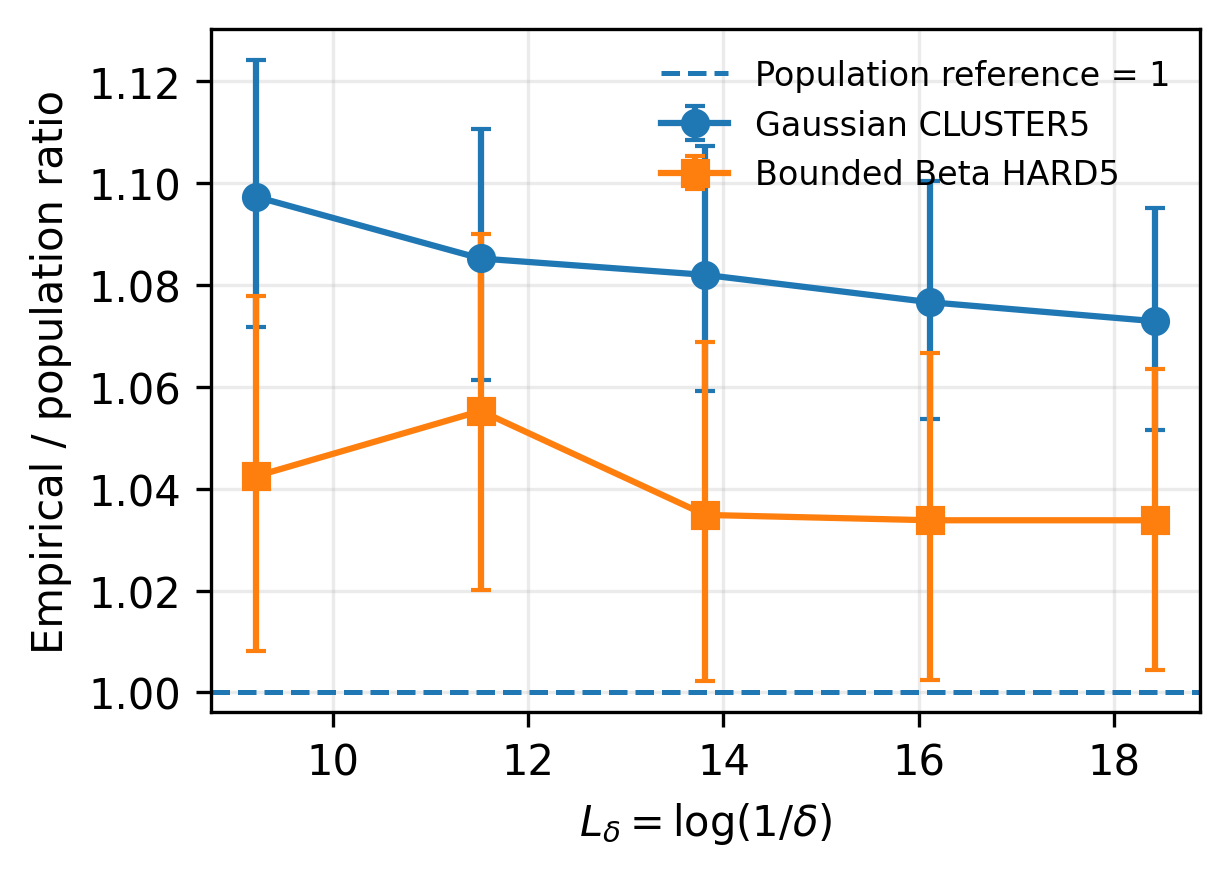
\includegraphics[width=\columnwidth]{figures/main_relative_efficiency_combined.png}
\caption{\textbf{Relative full-versus-one-bit efficiency.}
For Gaussian CLUSTER5 and bounded Beta HARD5 at $\beta=.5$, we plot
$R_{\rm rel}(\delta)=
(\overline\tau_{\rm 1bit}/\overline\tau_{\rm full})/
(T^\star_{\rm 1bit}/T^\star_{\rm full})$.
Intervals are 95\% paired-bootstrap confidence intervals over replication IDs.
The dashed reference at one represents agreement with the \emph{population
relative} characteristic-time prediction; it is not a finite-$\delta$ bound.}
\label{fig:relative-efficiency}
\end{figure}

\begin{figure}[t]
\centering
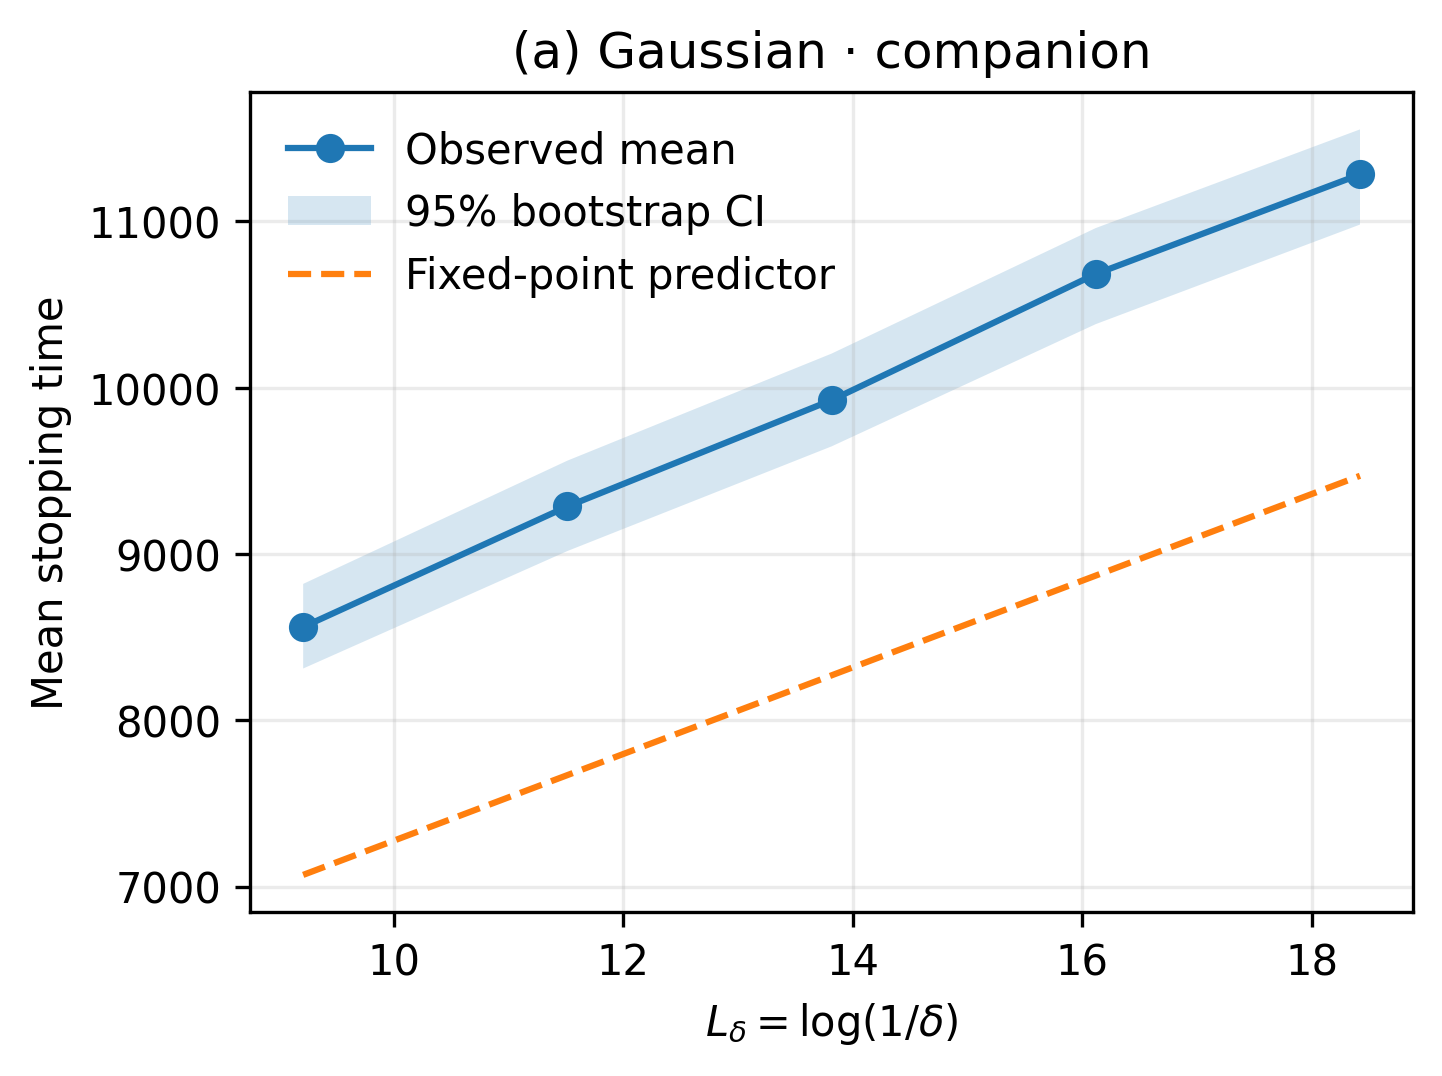
\includegraphics[width=\linewidth]{figures/main_calibration_E_companion.png}\\[-1mm]
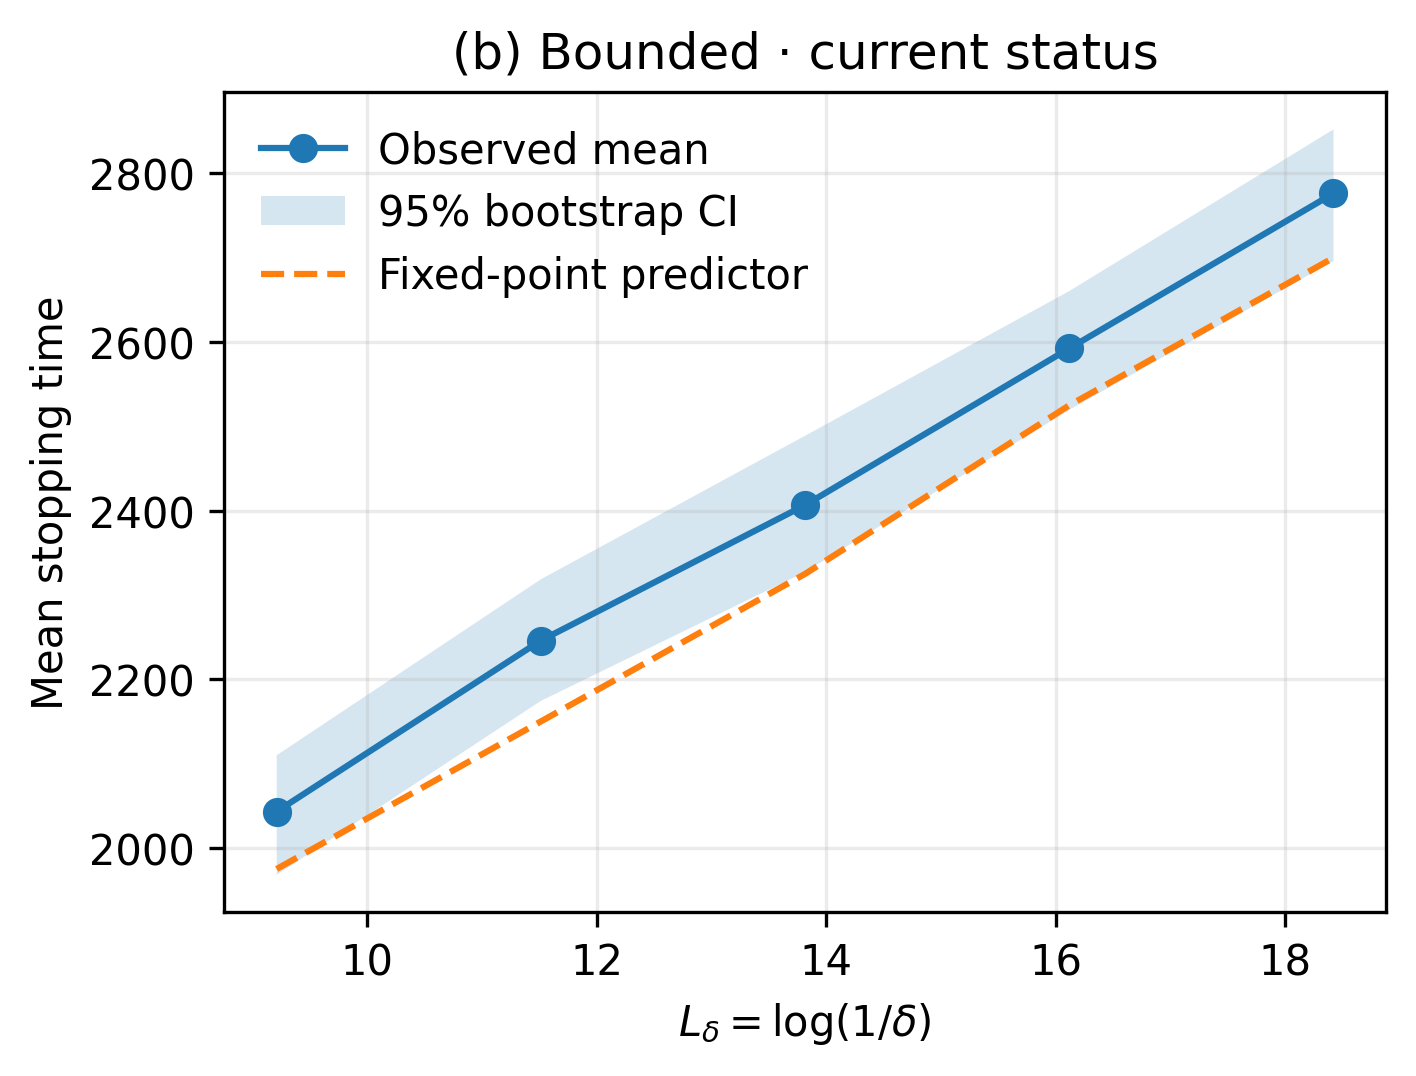
\includegraphics[width=\linewidth]{figures/main_calibration_U_raw.png}
\caption{\textbf{Practical one-bit finite-confidence calibration.}
Top: the separate Gaussian identification-schedule companion.
Bottom: bounded raw current-status one-bit.
Solid curves show empirical mean stopping times; dashed curves show the
fixed-point predictor~\eqref{eq:practical-predictor}; shaded regions are
bootstrap 95\% confidence intervals.  These use practical implementation
boundaries, not the certified non-asymptotic upper bounds.}
\label{fig:practical-calibration}
\end{figure}

\paragraph{Protocol.}
We use synthetic Gaussian and bounded instances to test three aspects of the
theory: the relative information loss caused by one-bit feedback, direct
first-order behavior, and finite-confidence calibration of practical stopping
rules.  Model E uses Gaussian rewards with known $\sigma=0.2$ and compares
full-feedback Top--Two with adaptive \emph{shared-threshold} one-bit Top--Two.
Model U uses Beta laws only as bounded reward generators; the full-feedback
baseline is nonparametric, while the one-bit method retains the raw
current-status observation $(Q,Y)$ with $Q\sim{\rm Unif}[0,1]$.
Full and one-bit replications are paired by instance, confidence level, and
replication identifier for lower-variance ratio estimates.  Appendix~\ref{app:experiments}
gives the complete grids, seeds, caps, correctness checks, and stress runs.

\paragraph{Relative efficiency and first-order behavior.}
Figure~\ref{fig:relative-efficiency} compares the empirical one-bit/full
stopping-time ratio with the corresponding ratio of population characteristic
times.  The normalized ratio is already near one on the representative
five-arm instances, indicating that the population characteristic times
capture most of the relative information loss.  This remains a \emph{relative}
diagnostic: finite-time overheads can partially cancel.  The supplement
therefore also reports the direct normalization
$\overline\tau_\delta/(T^\star\log(1/\delta))$ separately for full and one-bit
feedback and the deeper $\delta$ grid used to assess approach to the
first-order limit.

\paragraph{Practical finite-confidence calibration.}
For each one-bit implementation, define
\begin{equation}
n_{\rm pred}(\delta)
:=\min\{n\in\mathcal T:
 n\Gamma_{\rm 1bit}^{\rm pop}\ge b_{\rm prac}(n,\delta)\},
\label{eq:practical-predictor}
\end{equation}
where $\mathcal T$ is the implementation's stopping-check schedule and
$b_{\rm prac}$ is the practical simulation boundary.  This predicts the scale
of the implemented stopping time; it is neither an exact formula for
$\E[\tau_\delta]$ nor the numerical upper bound supplied by the certified
non-asymptotic theorems.  Figure~\ref{fig:practical-calibration} shows that the
predictor tracks the raw current-status stopping scale more closely than the
Gaussian companion on the archived benchmark.  The distinction matters
because the Gaussian $2/3$ result belongs to a separate companion policy,
whereas the practical raw-U boundary is not the paper-certified sieve
boundary.

\paragraph{Takeaway.}
Population characteristic times describe the instance-dependent information
loss, while the fixed-point predictor captures finite-confidence implementation
overhead.  The fixed/shared/pairwise distinction in Model E remains theoretical:
shared is the feasible joint $K$-arm design, while pairwise is a relaxation.

% ================= END OF 8-PAGE MAIN TEXT =================
